\documentclass[12pt]{article}
\usepackage{amsmath}
\usepackage{amssymb}
\usepackage{amsthm}
\usepackage{amsfonts}
\usepackage{graphicx}
\usepackage{textcomp}
\usepackage{hyperref}
\usepackage{tikz}
\usepackage{enumitem}
\usepackage{mathtools}
\usepackage{enumitem}
\usepackage{wasysym}
\usepackage{ulem}
\usepackage{xspace}
\usepackage{csquotes}

\DeclareMathOperator{\dist}{dist}
\DeclareMathOperator{\Nul}{Nul}
\DeclareMathOperator{\Row}{Row}
\DeclareMathOperator{\proj}{proj}

\begin{document}

\setlength{\arraycolsep}{12pt}

\newcommand{\defn}{\textbf{Def.}\xspace}
\newcommand{\thm}{\textbf{Thm.}\xspace}
\newcommand{\ex}{\textbf{Ex.}\xspace}
\renewcommand{\arraystretch}{1.25} % Adjust row spacing

\title{MACM 316 Lecture 12}
\author{Alexander Ng}
\date{Friday, January 31, 2025}

\maketitle

\subsubsection*{Example 1}

Prove that $x^{(k)} = \left(\frac{1}{k}, 1+e^{1-k}, -\frac{2}{k^2}\right)^t$
is convergent w.r.t. $||\cdot||_2$.

We know $0 \leq ||x^{(k)}-x||_2 \leq \sqrt{3}||x^{(k)}-x||_{\infty}$

\begin{eqnarray*}
  \lim_{k \to \infty} ||x^{(k)}-x||_{\infty} = 0 \implies \lim_{k \to \infty}
  ||x^{(k)}-x||_2 = 0 \\
\end{eqnarray*}

So, $\left\{x^{(k)}\right\}$ is convergent to $x$ w.r.t. $||\cdot||_2$.

It can be shown that \uline{all} norms on $\mathbb{R}^n $ are equivalent with
respect to convergence.

i.e. If $||\cdot||_a$ and $||\cdot||_b$ are norms on $\mathbb{R}^n$, and
$\left\{x^{(k)}\right\}_{k=1}^{\infty}$ has the limit $x$ with respect to
$||\cdot||_a$, then $\left\{x^{(k)}\right\}_{k=1}^{\infty}$ also has the limit
$x$ with respect to $||\cdot||_b$.

\section{Matrix Norms}

\textbf{Def.} A \uline{matrix norm} on the set of all $n \times n$ matrices 
$(R^{n \times n})$ is a real-valued function $||\cdot||$ defined on this set
satisfying for all $n \times n$ matries $A$ and $B$ and all real numbers
$\alpha:$

\begin{enumerate}
  \item $||A|| \geq 0$
  \item $||A|| = 0 \iff A=0$
  \item $||\alpha A|| = |\alpha| ||A||$
  \item $||A+B|| \leq ||A|| + ||B||$
  \item $||AB|| \leq ||A|| ||B||$
\end{enumerate}

\textbf{Def.} A distance between two $n\times n$ matrices $A$ and $B$ is

\begin{equation*}
  ||A-B||
\end{equation*}

\subsection{Thm.}

If $||\cdot||$ is a vector norm on $\mathbb{R}^n $, then 

\begin{equation*}
  ||A|| = \max_{||x||=1} ||Ax||.
\end{equation*}

is a matrix norm.

This is called the natural or induced matrix norm associated with the vector
norm.

The following result gives a bound on the value of $||Ax||$:

\subsection{Thm.}

For any vector $x\ne 0$, matrix $A$, and any natural norm $||\cdot||$, we have

\begin{equation*}
  ||Ax|| \leq ||A|| \cdot ||x||.
\end{equation*}

\subsubsection{Notes on the Infinity Norm}

The infinity norm is defined as

\begin{equation*}
  ||x||_\infty = \max_{i} |x_i|
\end{equation*}

So, it's the maximum absolute value of every entry in $x$.

\textbf{Example:} $x=\left(\begin{array}{c}
  1 \\
  -2 \\
  1.5 \\
\end{array}\right)$

$||x||_\infty = 2$

Because the largest element (in magnitude) is $-2$.

\section{Computing the Infinity Norm and the 1-Norm}

Computing the $\infty$-norm of a matrix is straightforward:

\subsection{Thm.}

If $A=(a_{ij})$ is a $n \times n$ matrix, then

\begin{equation*}
  ||A||_\infty = \max_{1\leq i \leq n} \sum_{j=1}^n |a_{ij}|
\end{equation*}

\textbf{Example:}

Find 

\begin{equation*}
  \left|\left| \begin{bmatrix}
  2 & -1 & 0\\
  -1 & 2 & -1\\
  0 & -1 & 2\\
  \end{bmatrix} \right|\right|_\infty
\end{equation*}

\begin{align*}
  \sum_{j=1}^n |a_{1j}| &= |2| + |-1| + |0| = 3 \\
  \sum_{j=1}^n |a_{2j}| &= |-1| + |2| + |-1| = 4 \\
  \sum_{j=1}^n |a_{3j}| &= |0| + |-1| + |2| = 3 \\
  \implies ||A||_\infty &= \max\{3, 4, 3\} = 4
\end{align*}

\pagebreak
\subsection{Visualizing the Infinity Norm}

Images courtesy of ChatGPT. I got really confused by the concept of the
infinity norm, so I asked the bot for help.

\begin{figure}[h]
  \centering
  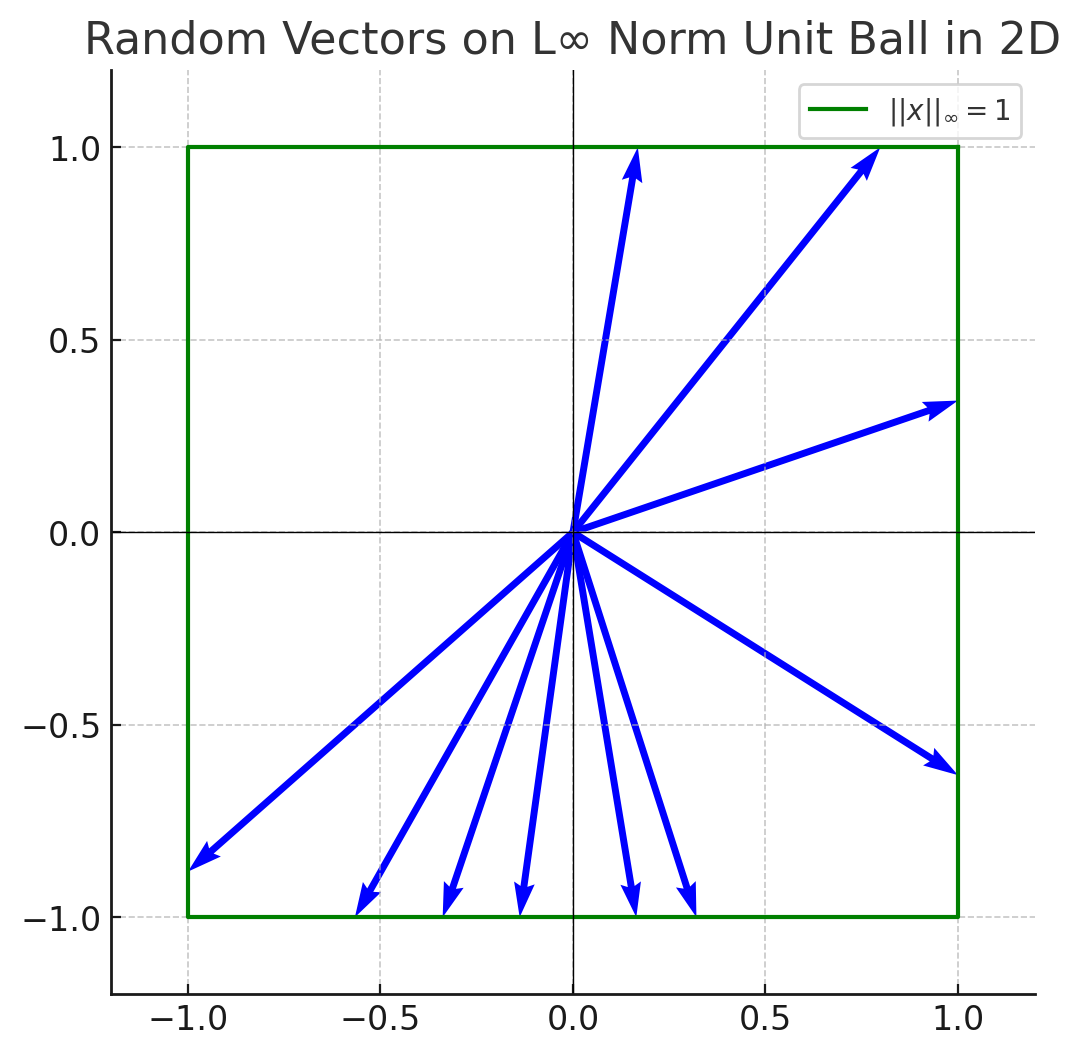
\includegraphics[width=0.8\textwidth]{./infinity_norm.png}
  \caption{Visualizing the Infinity Norm}
\end{figure}

So the reason why the infinity norm, visualized this way,
looks like a square, is because the equation $||x||_\infty = 1$ is equivalent 
to saying \enquote{the set of all vectors $x$ such that the the largest 
component magnitude of the vector is 1}. Meaning this is the set of all vectors
that have $x=1$ or $y=1$

\section{Eigenvalues and Eigenvectors} % spend time reviewing this

To calculate the $l_\infty$-norm of a matrix, we did not need to directly
appy the definition. This is also true for the $l_2$-norm, however, we will need
to introduce eigenvalues and eigenvectors to apply this technique.

First we will need the following definition:

\noindent
\textbf{Def.} If $A$ is a square matrix, the polynomial defined by

\begin{equation*}
  p(\lambda) = \det(A-\lambda I)
\end{equation*}

\noindent
\hangindent=0.5cm
\hangafter=0
is called the \uline{characteristic polynomial} of $A$. It is easily shown that
$p$ is an $n^{th}$ degree polynomial.

Now we can introduce eigenvalues and eigenvectors.

\noindent
\hangindent=0.5cm
\hangafter=1
\textbf{Def.} If $p$ is the characteristic polynomial of the matrix $A$, the
zeros of $p$ are called eigenvalues, or characteristic values of $A$. If $
\lambda$ is an eigenvalue of $A$ and $x\ne 0$ has the property that 
$(A-\lambda I)x = 0$ then $x$ is called an eigenvector, or characteristic
vector, of $A$ corresponding to the eigenvalue $\lambda$.

\noindent\rule{\linewidth}{0.5pt}

The professor does not specifically discuss eigenvectors and eigenvalues in the
context of Numerical Analysis, but they will be important for future problems.
He also does not mention how to compute them.

However, he did suggest that we review how to compute them by hand and study 
the related theorems.

\section{Finding the $l_2$-norm of a matrix}

\defn The spectral radius $\rho(A)$ of a matrix $A$ is defined as

\begin{equation*}
  \rho(A) = \max \left|\lambda\right| \text{ where } \lambda \text{ is an eigenvalue of } A
\end{equation*}

\ex

\begin{equation*}
  \rho(\begin{bmatrix}
  2 & 1 & 0\\
  1 & 2 & 0\\
  0 & 0 & 3\\
  \end{bmatrix}) = \max \left\{ |3|, |3|, |1| \right\} = 3
\end{equation*}

And now, we can consider the following:

\pagebreak
\thm If $A$ is a $n \times n$ matrix, then

\begin{enumerate}
  \item $||A||_2 = \sqrt{\rho(A^T A)}$
  \item $\rho(A) \leq ||A||$ for any natural norm $||\cdot||$
\end{enumerate}

My editor broke in the middle so you should look at the Chapter 7 PDF notes
for the proofs and examples. The end of this section is around page 19 of 
the PDF. (35.13)

\end{document}
